\documentclass{article}
\usepackage[utf8]{inputenc}
\usepackage{amsmath}
\usepackage{graphicx}
\title{Homework 3 Solution}
\author{Qazi Umer Jamil }
% 34 MTS B%
%EE379 - Linear Control Systems (LCS)%
\date{January 15, 2016}

\begin{document}

\maketitle

\section{Solution of Problem 2 through PID Controller Design}

System parameters are as follows:
\[M = 2.87\]
\[m = 0.9\]
\[b = 0.5\]
\[I = 0.005\]
\[g = 9.8\]
\[l = 3.12\]
\[Ts = 7\]
\[Re = -4/Ts\]
\[\theta = 0.005\]
\[q = (M+m)*(I+m*l^2)-(m*l)^2\]
The transfer function of cart is
\[Pcart = \frac{(((I+m*l^2)/q)*s^2 - (m*g*l/q))}{(s^4 + (b*(I + m*l^2))*s^3/q - ((M + m)*m*g*l)*s^2/q - b*m*g*l*s/q)} \]

\[Ppend = \frac{(m*l*s/q)}{(s^3 + (b*(I + m*l^2))*s^2/q - ((M + m)*m*g*l)*s/q - b*m*g*l/q)} \]

Here we are only interested in the control of the pendulum's position. We don't care the velocity or other parameters of cart.

Design requirements for this system are:
1. Settling time for theta of less than 5 seconds
2. Pendulum angle theta never more than 0.05 radians from the vertical
3. Steady State error less then 3 sec

The root locus of our uncompensated system is shown in Figure 1.
\begin{figure}[h]
  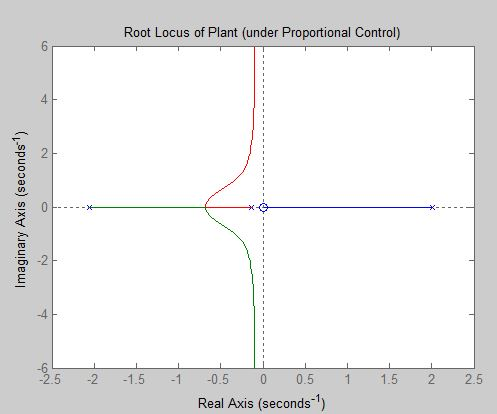
\includegraphics[width=\linewidth]{fig1.JPG}
  \caption{Root Locus of uncompensated system}
  \label{fig:boat1}
\end{figure}
As one of the branches of the above root locus is entirely in the right-half plane. This means that will always be a closed-loop pole in the right-half plane, thus making the system's impulse response unstable. To solve this problem, we need to add a pole at the origin (an integrator) via the controller to cancel the plant zero at the origin. This addition will produce two closed-loop poles in the right-half plane. 
In our subsequent design we can then modify our controller to draw these poles into the left-half plane, thereby stabilizing the closed-loop system. So, adding a pole at origin, the root locus take the form as shown in Figure 2.
\begin{figure}[h]
  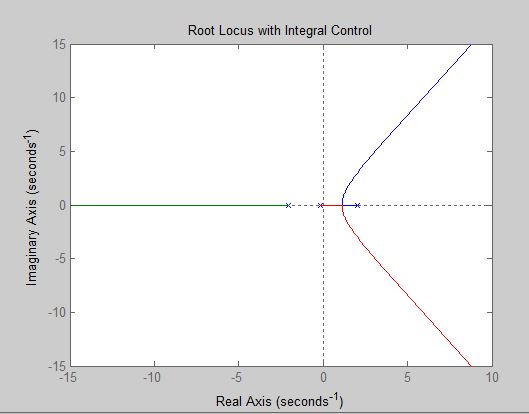
\includegraphics[width=\linewidth]{fig2.JPG}
  \caption{Root Locus with Integral Control}
  \label{fig:boat1}
\end{figure}

So now we want to draw the root locus branches into the left-half plane to make the system stable. 
Using MATLAB, the pole and zeros of our system are as follows:
\[zeros = 0\]
\[poles = 0, 2.0111, -2.0528, -0.1324 \]
\\
So, there are four poles and only one zero. This means that the root locus will have three asymptotes: 
1. One along the real axis in the negative direction
2. The other two at 120 degree angles to this one.

This configuration is also unsatisfactory because we still have branches of the root locus that are entirely in the right-half complex plane. In general, we can pull the branches of our root locus to the left in the complex plane by adding zeros to our system. Adding a zero to our controller will reduce the number of asymptotes from three to two.
\\
So adding a zero to our integral controller could pull the branches of the root locus to the left in the complex plane, but we were not able to the pull the dominant branches far enough to the left. A possible solution is to add yet another zero. If we place both zeros on the negative real axis between the two plant poles, then the two branches in the right-half plane will be pulled into the left-half plane and will terminate at these two zeros. Let's specifically evaluate the root locus for a controller with an integrator and zeros at -1, -0.5 The compensator will be \[\frac{(s+1)(s+0.5)}{s}\]. The root locus of compensated system is shown in figure 3.
\begin{figure}[h]
  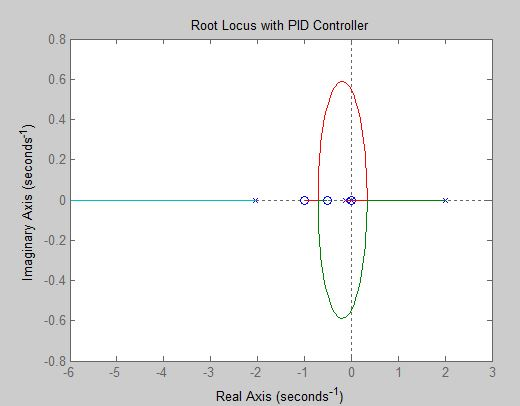
\includegraphics[width=\linewidth]{fig3.JPG}
  \caption{Root Locus with PID Controller}
  \label{fig:boat1}
\end{figure}


Examining the above root locus helps us to determine whether or not our given requirements can be met. Specifically, since it is desired that the settling time of the system be less than 7 seconds, the real parts of our dominant closed-loop poles should be less than approximately 
\[\frac{-4}{7} = -0.571\]

In other words, our dominant closed-loop poles should be located in the complex to the left of a vertical line at s = -0.571. Since it is also desired that the pendulum not move more than 0.06 radians away from vertical, we also want to ensure that the closed-loop system has sufficient damping. Placing the dominant closed-loop poles near the real axis will increase the system's damping.

The  gain corresponding to a specific point on the root locus can be found using a MATLAB command as follows
\[[k,poles] = rlocfind(C*Ppend)\]

\[selected_point = -0.7087 + 0.0011i\]
\[k =310.5155\]
\[zeros = 0\]
\[poles =0,-33.4083 + 0.0000i, -0.7087 + 0.0011i, -0.7087 - 0.0011i\]


The impulse response of our closed-loop system is shown in figure 4.

\begin{figure}[h]
  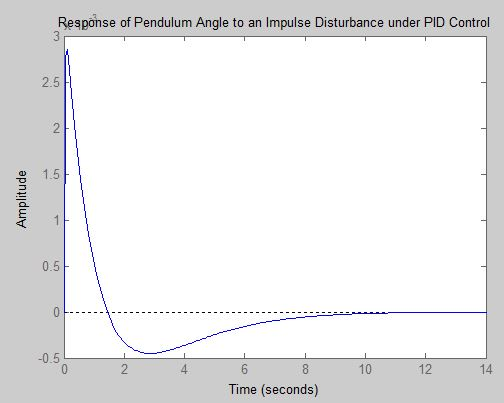
\includegraphics[width=\linewidth]{fig4.JPG}
  \caption{Impulse response of PID compensated system}
  \label{fig:boat1}
\end{figure}



\section{Solution of Problem 2 through Lead-Lag Controller Design}


Continue the discussion after implementing the PID Controller, the root locus entirely shift to the left half plane if we place a pole at -0.2 and zeros at -1 -0.5.

The compensator will be
\[ \frac{(s+1)(s+0.5)}{(s+0.2)}\]

\begin{figure}[h]
  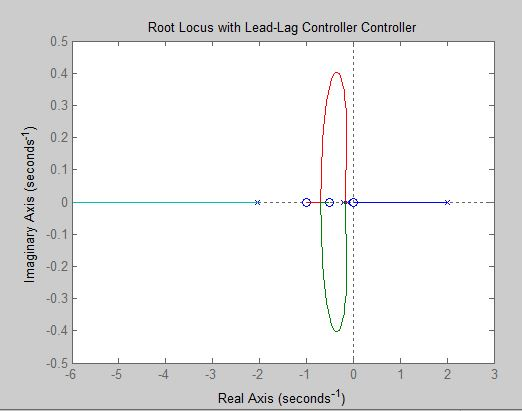
\includegraphics[width=\linewidth]{fig6.JPG}
  \caption{Root Locus with Lead-Lag Controller Controller}
  \label{fig:boat1}
\end{figure}

To find the gain corresponding to a specific point on the root locus, we can use the rlocfind command.  The  gain corresponding to a specific point on the root locus can be found using a MATLAB command as follows
\[[k,poles] = rlocfind(C*Ppend)\]


\[selected-point = -0.6905 + 0.0000i\]
\[k = 221.7485\]
\[zeros = 0\]
\[poles = -23.7485 + 0.0000i, -0.6905 + 0.0000i, -0.6905 - 0.0000i, 0.0097 + 0.0000i\]

The impulse response of our closed-loop system is shown in figure 6.

\begin{figure}[h]
  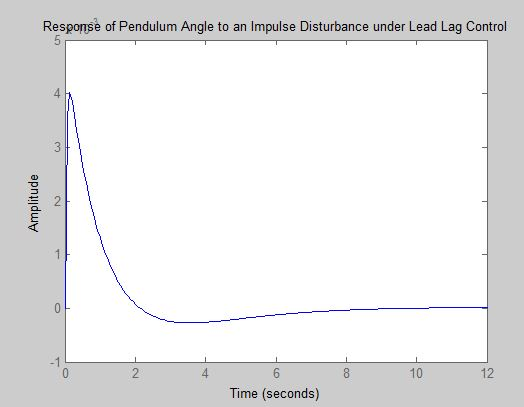
\includegraphics[width=\linewidth]{fig5.JPG}
  \caption{Impulse response of Lead-Lag compensated system.}
  \label{fig:boat1}
\end{figure}

\section{References}
    1. http://ctms.engin.umich.edu/CTMS/index.php

\end{document}
